% Options for packages loaded elsewhere
\PassOptionsToPackage{unicode}{hyperref}
\PassOptionsToPackage{hyphens}{url}
%
\documentclass[
]{book}
\usepackage{lmodern}
\usepackage{amssymb,amsmath}
\usepackage{ifxetex,ifluatex}
\ifnum 0\ifxetex 1\fi\ifluatex 1\fi=0 % if pdftex
  \usepackage[T1]{fontenc}
  \usepackage[utf8]{inputenc}
  \usepackage{textcomp} % provide euro and other symbols
\else % if luatex or xetex
  \usepackage{unicode-math}
  \defaultfontfeatures{Scale=MatchLowercase}
  \defaultfontfeatures[\rmfamily]{Ligatures=TeX,Scale=1}
\fi
% Use upquote if available, for straight quotes in verbatim environments
\IfFileExists{upquote.sty}{\usepackage{upquote}}{}
\IfFileExists{microtype.sty}{% use microtype if available
  \usepackage[]{microtype}
  \UseMicrotypeSet[protrusion]{basicmath} % disable protrusion for tt fonts
}{}
\makeatletter
\@ifundefined{KOMAClassName}{% if non-KOMA class
  \IfFileExists{parskip.sty}{%
    \usepackage{parskip}
  }{% else
    \setlength{\parindent}{0pt}
    \setlength{\parskip}{6pt plus 2pt minus 1pt}}
}{% if KOMA class
  \KOMAoptions{parskip=half}}
\makeatother
\usepackage{xcolor}
\IfFileExists{xurl.sty}{\usepackage{xurl}}{} % add URL line breaks if available
\IfFileExists{bookmark.sty}{\usepackage{bookmark}}{\usepackage{hyperref}}
\hypersetup{
  pdftitle={Biostatistika Inferensial},
  pdfauthor={dimas \& ulya},
  hidelinks,
  pdfcreator={LaTeX via pandoc}}
\urlstyle{same} % disable monospaced font for URLs
\usepackage{longtable,booktabs}
% Correct order of tables after \paragraph or \subparagraph
\usepackage{etoolbox}
\makeatletter
\patchcmd\longtable{\par}{\if@noskipsec\mbox{}\fi\par}{}{}
\makeatother
% Allow footnotes in longtable head/foot
\IfFileExists{footnotehyper.sty}{\usepackage{footnotehyper}}{\usepackage{footnote}}
\makesavenoteenv{longtable}
\usepackage{graphicx,grffile}
\makeatletter
\def\maxwidth{\ifdim\Gin@nat@width>\linewidth\linewidth\else\Gin@nat@width\fi}
\def\maxheight{\ifdim\Gin@nat@height>\textheight\textheight\else\Gin@nat@height\fi}
\makeatother
% Scale images if necessary, so that they will not overflow the page
% margins by default, and it is still possible to overwrite the defaults
% using explicit options in \includegraphics[width, height, ...]{}
\setkeys{Gin}{width=\maxwidth,height=\maxheight,keepaspectratio}
% Set default figure placement to htbp
\makeatletter
\def\fps@figure{htbp}
\makeatother
\setlength{\emergencystretch}{3em} % prevent overfull lines
\providecommand{\tightlist}{%
  \setlength{\itemsep}{0pt}\setlength{\parskip}{0pt}}
\setcounter{secnumdepth}{5}
\usepackage{booktabs}
\usepackage{amsthm}
\makeatletter
\def\thm@space@setup{%
  \thm@preskip=8pt plus 2pt minus 4pt
  \thm@postskip=\thm@preskip
}
\makeatother
\usepackage[]{natbib}
\bibliographystyle{apalike}

\title{Biostatistika Inferensial}
\author{dimas \& ulya}
\date{2021-03-05}

\begin{document}
\maketitle

{
\setcounter{tocdepth}{1}
\tableofcontents
}
\hypertarget{pengantar}{%
\chapter{Pengantar}\label{pengantar}}

Modul ini dibuat sebagai bahan ajar pada mata kuliah Biostatistika Inferensial Fakultas Kesehatan Masyarakat Universitas Jember. Pada buku ini akan membahas beberapa topik perkuliahan yaitu:

\begin{itemize}
\tightlist
\item
  Uji 2 sampel independen
\item
  Uji 2 sampel berpasangan
\item
  Uji Anova
\item
  Uji Korelasi
\item
  Uji Regresi Linier
\end{itemize}

\hypertarget{uji2sampelind}{%
\chapter{Uji 2 Sampel Independen}\label{uji2sampelind}}

\hypertarget{tujuan}{%
\section{Tujuan}\label{tujuan}}

\begin{itemize}
\tightlist
\item
  Mahasiswa mampu memahami konsep dasar pengujian 2 sampel independen
\item
  Mahasiswa mampu melakukan melakukan pengujian 2 sampel independen secara manual
\item
  Mahasiswa mampu melakukan melakukan pengujian 2 sampel independen menggunakan aplikasi pengolah data
\end{itemize}

\hypertarget{dasar-teori}{%
\section{Dasar Teori}\label{dasar-teori}}

Terkadang kita ingin mengetahui apakah sebuah kelompok data (sampel data) memiliki nilai rata-rata yang sama dengan kelompok data yang lain. Tentu kata ``sama'' dalam hal ini tidak memiliki arti sama persis sebab hal ini sangat jarang terjadi. Akan selalu ada kesalahan yang dapat ditolernasi di setiap pengujian.

Andaikan dari 10 sampel mahasiswa laki-laki diperoleh rata-rata tinggi badan = 168,5 dan dari 10 sampel mahasiswa perempuan diperoleh tinggi badan = 167,2. Apakah dapat disimpulkan bahwa tinggi badan mahasiswa laki-laki = tinggi badan mahasiswa perempuan? Jika ``ya'', maka apa dasar pengambilan kesimpulan tersebut?

Uji 2 sampel independen merupakan uji statistik yang digunakan untuk menguji nilai rata-rata dari 2 kelompok/sampel/populasi yang saling bebas. Terdapat 2 pengujian yang dapat dilakukan pada kasus ini, yang pertama adalah Uji t 2 Sampel Independen (parametrik) dan Uji Mann Whitney (non-parametrik).

Berikut ini adalah contoh kasus 2 sampel independen (yang saling bebas):

\begin{itemize}
\tightlist
\item
  Kepala Dinas Kesehatan ingin menguji apakah ada perbedaan jumlah kunjungan pada puskesmas yang berada di daerah perkotaan dan daerah pedesaan.
\item
  Seorang peneliti menduga bahwa terdapat perbedaan kandungan gizi antara roti tawar yang biasa dengan roti tawar yang telah ditambahkan dengan tepung kelor.
\item
  Perusahaan farmasi A meyakini bahwa produk obat penurun gula darah yang mereka produksi dapat menurunkan kadar gula lebih baik daripada produk dari perusahaan farmasi B
\end{itemize}

\hypertarget{hipotesis-pengujian}{%
\subsection{Hipotesis Pengujian}\label{hipotesis-pengujian}}

Terdapat 3 hipotesis yang dapat digunakan dalam melakukan pengujian dengan menggunakan Uji t 2 Sampel Independen.

\textbf{Hipotesis Satu Arah Kanan}\\
Hipotesis ini digunakan untuk menguji apakah rata-rata dari suatu sampel/kelompok lebih besar dari sampel/kelompok yang lain. Hipotesis ditulis sebagai berikut:\\
\(H_0 : \mu_1-\mu_2 \leq d_0\)\\
\(H_1 : \mu_1-\mu_2 > d_0\)

Apabila \(d_0 = 0\), maka hipotesis akan menjadi:\\
\(H_0 : \mu_1 \leq \mu_2\)\\
\(H_1 : \mu_1 > \mu_2\)

Daerah penolakan dan penerimaan \(H_0\) pada \(\alpha = 5\%\) dan \(df = 10000\) dapat dilihat pada gambar berikut:

\begin{center}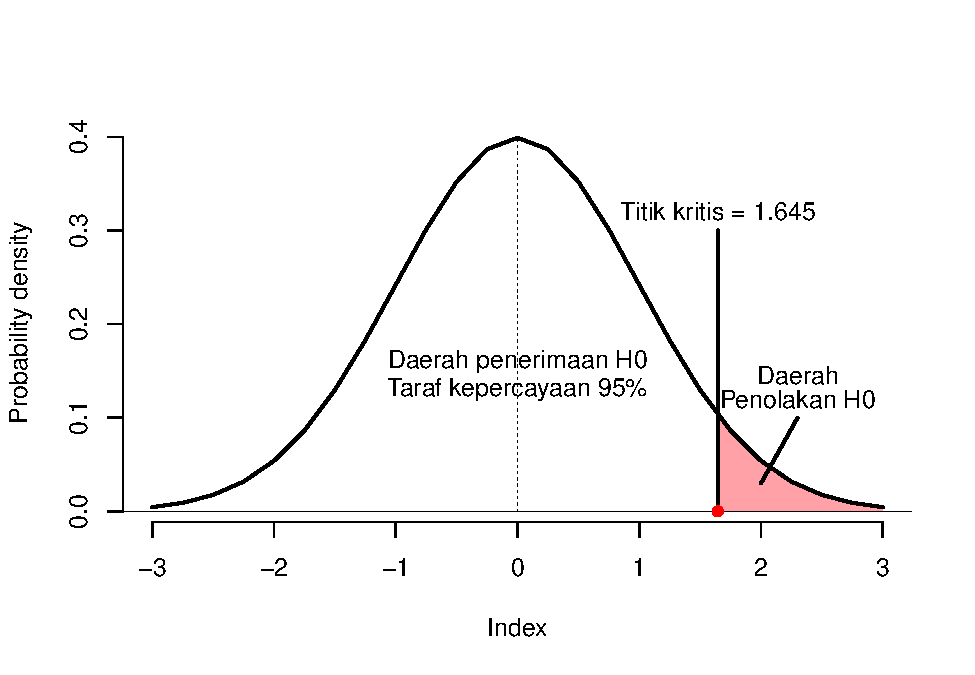
\includegraphics[width=0.75\linewidth,height=0.75\textheight]{biostatistika-inferensial_files/figure-latex/unnamed-chunk-2-1} \end{center}

Penolakan \(H_0\) dilakukan apabila nilai \(t_{hitung}\) berada pada daerah penolakan H0 (\(t_{hitung}\) \textgreater{} nilai kritis \(1.645\)).

\textbf{Hipotesis Satu Arah Kiri}\\
Hipotesis ini digunakan untuk menguji apakah rata-rata dari suatu sampel/kelompok lebih kecil dari sampel/kelompok yang lain. Hipotesis ditulis sebagai berikut:\\
\(H_0 : \mu_1-\mu_2 \geq d_0\)\\
\(H_1 : \mu_1-\mu_2 < d_0\)

Apabila \(d_0 = 0\), maka hipotesis akan menjadi:\\
\(H_0 : \mu_1 \geq \mu_2\)\\
\(H_1 : \mu_1 < \mu_2\)

Daerah penolakan dan penerimaan \(H_0\) pada \(\alpha = 5\%\) dan \(df = 10000\) dapat dilihat pada gambar berikut:

\begin{center}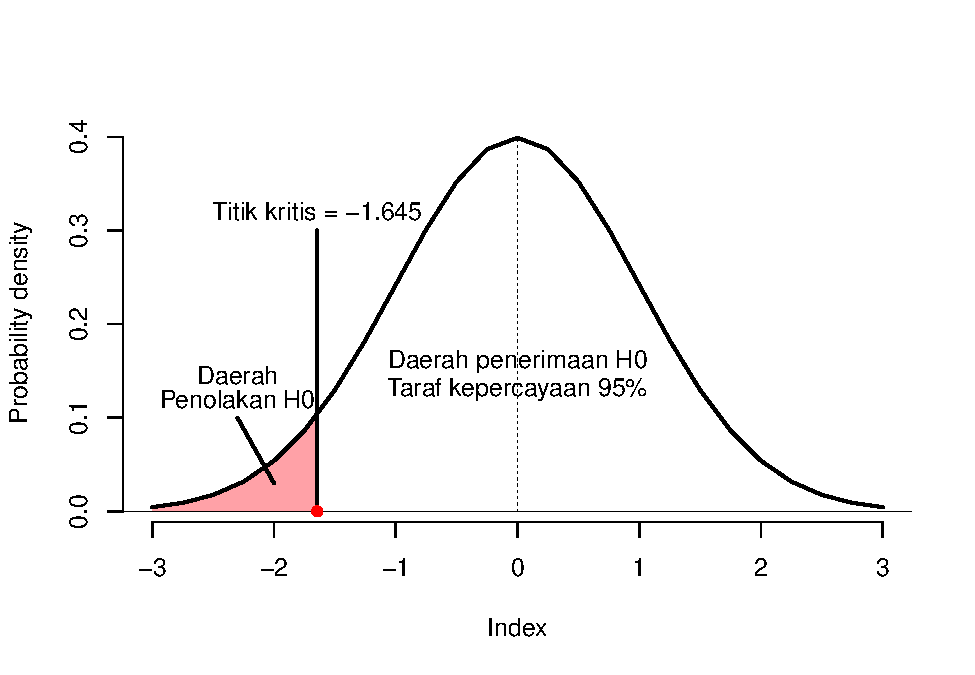
\includegraphics[width=0.75\linewidth,height=0.75\textheight]{biostatistika-inferensial_files/figure-latex/unnamed-chunk-4-1} \end{center}

Penolakan \(H_0\) dilakukan apabila nilai \(t_{hitung}\) berada pada daerah penolakan H0 (\(t_{hitung}\) \textless{} nilai kritis \(-1.645\)).

\textbf{Hipotesis Dua Arah}\\
Hipotesis ini digunakan untuk menguji apakah rata-rata dari suatu sampel/kelompok berbeda (dapat lebih besar atau lebih kecil) dari sampel/kelompok yang lain. Hipotesis ditulis sebagai berikut:\\
\(H_0 : \mu_1-\mu_2 = d_0\)\\
\(H_1 : \mu_1-\mu_2 \neq d_0\)

Apabila \(d_0 = 0\), maka hipotesis akan menjadi:\\
\(H_0 : \mu_1 = \mu_2\)\\
\(H_1 : \mu_1 \neq \mu_2\)

Daerah penolakan dan penerimaan \(H_0\) pada \(\alpha = 5\%\) dan \(df = 10000\) dapat dilihat pada gambar berikut:

\begin{center}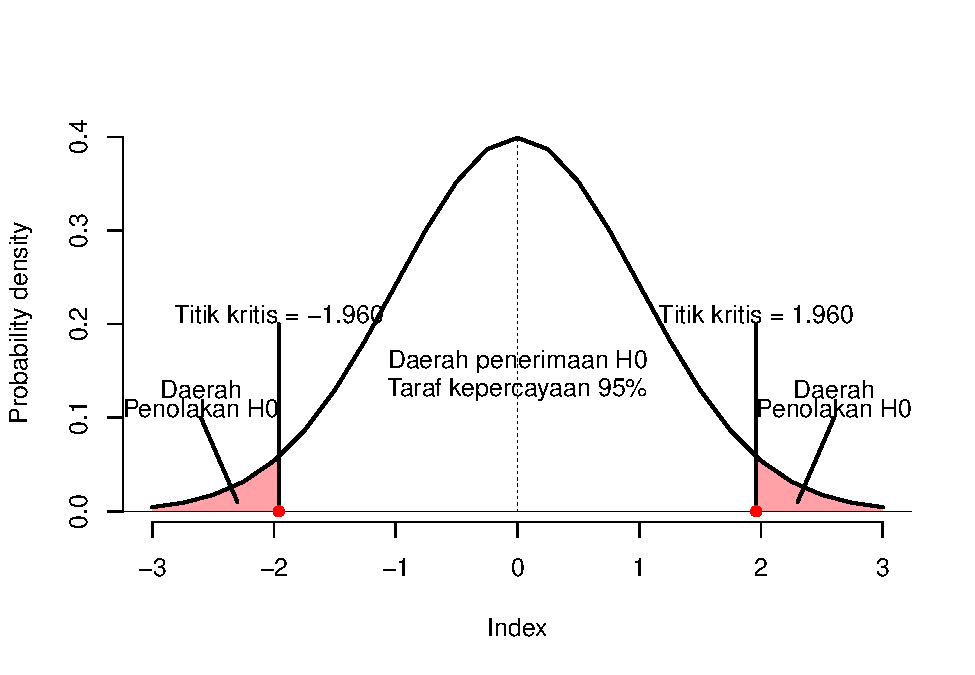
\includegraphics[width=0.75\linewidth,height=0.75\textheight]{biostatistika-inferensial_files/figure-latex/unnamed-chunk-6-1} \end{center}

Penolakan \(H_0\) dilakukan apabila nilai \(t_{hitung}\) berada pada daerah penolakan H0 (\(t_{hitung}\) \textless{} nilai kritis \(-1.960\) bila \(t_{hitung}\) negatif atau \(t_{hitung}\) \textgreater{} nilai kritis \(1.960\) bila \(t_{hitung}\) positif).

\hypertarget{uji-t-2-sampel-independen}{%
\subsection{Uji t 2 Sampel Independen}\label{uji-t-2-sampel-independen}}

Uji t 2 Sampel Independen memiliki beberapa asumsi yang harus terpenuhi, yaitu:

\begin{itemize}
\tightlist
\item
  Sampel/kelompok diambil secara acak
\item
  Sampel/kelompok independen
\item
  Sampel/kelompok berasal dari populasi yang berdistribusi normal
\item
  Memiliki varians antar sampel/kelompok yang sama (homogen)
\end{itemize}

Namun pada kasus kedua sampel tidak memiliki varians yang sama (homogen), uji dapat dilanjutkan dengan menggunakan derajat kebebasan yang berbeda.

Formula untuk Uji t 2 Sampel Independen (\(t_{hitung}\)) dengan asumsi varians antar kelompok sama ialah sebagai berikut \citep{allan18}:
\[
t = \frac{(\bar{X_1}-\bar{X_2})-(\mu_1-\mu_2)}{\sqrt{\frac{\sigma_1^2}{n_1}+\frac{\sigma_2^2}{n_2}}}
\]
dimana:

\begin{itemize}
\tightlist
\item
  derajat kebebasan sama dengan \(n-1\) (pada kasus \(n_1\) dan \(n_2\) yang sama)
\item
  pada kasus varians populasi (\(\sigma^2\)) tidak diketahui maka \(\sigma^2 = s^2 = \frac{\sum(x_i-\mu)}{n-1}\).
\end{itemize}

Selain itu, \(t_{hitung}\) juga dapat dihitung dengan formula berikut:
\[
t = \frac{(\bar{X_1}-\bar{X_2})-(\mu_1-\mu_2)}{s_p\sqrt{\frac{1}{n_1}+\frac{1}{n_2}}}
\]
dimana \(s_p = \sqrt{\frac{(n_1-1)s^2_1+(n_2-1)s^2_2}{n_1+n_2-2}}\).

Apabila hasil pengujian varians dinyatakan bahwa kedua sampel/kelompok tidak memiliki varians yang sama (homogen), maka derajat kebebasan dihitung dengan formula berikut:
\[
d.f = \frac{(s_1^2/n_1+s_2^2/n_2)^2}{(s_1^2/n_1)^2/(n_1-1)+(s_2^2/n_2)^2/(n_2-1)}
\]

\hypertarget{contoh}{%
\subsubsection{Contoh}\label{contoh}}

Berikut adalah contoh-contoh pengujian dengan menggunakan Uji t 2 Sampel Independen

\hypertarget{kasus-1}{%
\paragraph{Kasus 1}\label{kasus-1}}

Diketahui bahwa dalam 8 kali percobaan, rata-rata Ani dapat mengetik sebanyak 105 kata dengan standar deviasi 7 kata dalam waktu 1 menit. Dengan jumlah percobaan yang sama dengan Ani, Rudi dapat mengetik dengan rata-rata 115 kata dengan standar deviasi 10 dalam waktu 1 menit. Dengan menggunakan \(\alpha\) sebesar 5\%, apakah dapat disimpulkan bahwa Rudi dapat mengetik lebih cepat daripada Ani? Varians antar kelompok diasumsikan homogen.

\textbf{Jawab}\\

\begin{table}

\caption{\label{tab:unnamed-chunk-7}Deskriptif Kemampuan Mengetik Anis dan Rudi}
\centering
\begin{tabular}[t]{ccc}
\toprule
Statistik & Ani & Rudi\\
\midrule
n & 8 & 8\\
rata-rata & 105 & 115\\
standar deviasi & 7 & 10\\
\bottomrule
\end{tabular}
\end{table}

\emph{Langkah-langkah pengerjaan}

\begin{enumerate}
\def\labelenumi{\arabic{enumi}.}
\tightlist
\item
  Tentukan hipotesis pengujian:\\
  \(H_0 : \mu_1 \leq \mu_2\)\\
  \(H_1 : \mu_1 > \mu_2\)\\
  dimana \(\mu_1\) adalah rata-rata mengetik Rudi (populasi) dan \(\mu_2\) adalah rata-rata mengetik Ani (populasi)
\item
  Hitung derajat kebebasan \(dk = n - 1 = 8 - 1 = 7\).
\item
  Tentukan nilai \(t_{tabel}\) dengan \(\alpha=0.05\) dan \(dk = 7\), sehingga \(t_{(0.05,7)} = 1,8946\).
\item
  Hitung nilai \(t_{hitung}\) dengan menganggap bahwa \(\mu_1-\mu_2 = 0\), maka:\\
  \[
  t_{hitung} = \frac{(\bar{X_1}-\bar{X_2})}{\sqrt{\frac{s_1^2}{n_1}+\frac{s_2^2}{n_2}}}
  \]
  \[
  t_{hitung} = \frac{(115-105)}{\sqrt{\frac{10^2}{8}+\frac{7^2}{8}}} = 2,32
  \]
\item
  Bandingkan \(t_{hitung}\) dengan \(t_{tabel}\) (\(2,32 > 1,8946\)).
\item
  Pengambilan keputusan: Tolak \(H_0\) (karena \(t_{hitung}\) lebih besar dari \(t_{tabel}\)).
\end{enumerate}

Sehingga dapat disimpulkan bahwa dengan menggunakan \(\alpha = 5\%\) Rudi mengetik lebih cepat daripada Ani.

\hypertarget{kasus-2}{%
\paragraph{Kasus 2}\label{kasus-2}}

Dekan Fakultas XX menyatakan bahwa tekanan darah pria lansia lebih rendah daripada wanita lansia. Penelitian dilakukan untuk menguji teori tersebut dengan mengambil 20 pria dan 20 wanita lansia dan diukur tekanan darahnya. Hasil pengukuran menunjukkan bahwa rata-rata tekanan dara pria lansia adalah 115,6 dengan simpanan baku 7,3. Sedangkan hasil pengukuran pada wanita lansia menunjukkan rata-rata tekanan darah sebesar 121,5 dengan simpangan baku 11,2. Berdasarkan data tersebut, tentukan apakah pernyataan Dekan dapat dibenarkan dengan menggunakan \(\alpha=0.05\)?

\textbf{Jawab}\\

\begin{table}

\caption{\label{tab:unnamed-chunk-8}Deskriptif Data Pria dan Wanita Lansia}
\centering
\begin{tabular}[t]{ccc}
\toprule
Statistik & Pria & Wanita\\
\midrule
n & 20.0 & 20.0\\
rata-rata & 115.6 & 121.5\\
standar deviasi & 7.3 & 11.2\\
\bottomrule
\end{tabular}
\end{table}

\emph{Langkah-langkah pengerjaan}

\begin{enumerate}
\def\labelenumi{\arabic{enumi}.}
\tightlist
\item
  Tentukan hipotesis pengujian:\\
  \(H_0 : \mu_1 \geq \mu_2\)\\
  \(H_1 : \mu_1 < \mu_2\)\\
  dimana \(\mu_1\) adalah rata-rata pria lansia (populasi) dan \(\mu_2\) adalah rata-rata wanita lansia (populasi)
\item
  Hitung derajat kebebasan \(dk = n - 1 = 20 - 1 = 19\).
\item
  Tentukan nilai \(t_{tabel}\) dengan \(\alpha=0.05\) dan \(dk = 19\), sehingga \(t_{(0.05,19)} = -1,7291\).
\item
  Hitung nilai \(t_{hitung}\) dengan menganggap bahwa \(\mu_1-\mu_2 = 0\), maka:\\
  \[
  t_{hitung} = \frac{(\bar{X_1}-\bar{X_2})}{\sqrt{\frac{s_1^2}{n_1}+\frac{s_2^2}{n_2}}}
  \]
  \[
  t_{hitung} = \frac{(115.6-121.5)}{\sqrt{\frac{7.3^2}{20}+\frac{11.2^2}{20}}} = -6,44
  \]
\item
  Bandingkan \(t_{hitung}\) dengan \(t_{tabel}\) (\(-6,44<-1,7291\)).
\item
  Pengambilan keputusan: Tolak \(H_0\) (karena \(t_{hitung}\) lebih kecil dari \(t_{tabel}\)).
\end{enumerate}

Sehingga dapat disimpulkan bahwa dengan menggunakan \(\alpha = 5\%\) pernyataan Dekan Fakultas XX adalah benar.

\hypertarget{kasus-3}{%
\paragraph{Kasus 3}\label{kasus-3}}

Data berikut merupakan hasil penurunan berat badan dengan menggunakan Metode Diet A pada 10 responden wanita di wilayah perkotaan dan pedesaan.

\begin{table}

\caption{\label{tab:unnamed-chunk-9}Data Penurunan Berat Badan Wanita di Kota dan Desa}
\centering
\begin{tabular}[t]{cc}
\toprule
kota & desa\\
\midrule
3 & 5\\
3 & 6\\
5 & 6\\
4 & 5\\
5 & 5\\
\addlinespace
3 & 5\\
3 & 6\\
4 & 7\\
2 & 6\\
2 & 5\\
\bottomrule
\end{tabular}
\end{table}

Dengan menggunakan \(\alpha\) = 5\%, tentukan apakah ada perbedaan penurunan berat badan pada wanita di perkotaan dan pedesaan jika melakukan diet dengan menggunakan Metode Diet A?

\textbf{Jawab}\\

\begin{table}

\caption{\label{tab:unnamed-chunk-10}Deskriptif Data Penurunan Berat Badan Wanita di Desa dan di Kota}
\centering
\begin{tabular}[t]{ccc}
\toprule
Statistik & kota & desa\\
\midrule
n & 10.00 & 10.0\\
rata-rata & 3.40 & 5.6\\
standar deviasi & 1.07 & 0.7\\
\bottomrule
\end{tabular}
\end{table}

\emph{Langkah-langkah pengerjaan}

\begin{enumerate}
\def\labelenumi{\arabic{enumi}.}
\tightlist
\item
  Tentukan hipotesis pengujian:\\
  \(H_0 : \mu_1 = \mu_2\)\\
  \(H_1 : \mu_1 \neq \mu_2\)\\
  dimana \(\mu_1\) adalah rata-rata penurunan berat badan wanita di kota (populasi) dan \(\mu_2\) adalah rata-rata penurunan berat badan wanita di desa (populasi)
\item
  Hitung derajat kebebasan \(dk = n - 1 = 10 - 1 = 9\).
\item
  Tentukan nilai \(t_{tabel}\) dengan \(\alpha=0.05/2=0.025\) dan \(dk = 9\), sehingga \(t_{(0.025,9)} = -2,2622\) atau \(t_{(0.975,9)} = 2,2622\).
\item
  Hitung nilai \(t_{hitung}\) dengan menganggap bahwa \(\mu_1-\mu_2 = 0\), maka:\\
  \[
  t_{hitung} = \frac{(\bar{X_1}-\bar{X_2})}{\sqrt{\frac{s_1^2}{n_1}+\frac{s_2^2}{n_2}}}
  \]
  \[
  t_{hitung} = \frac{(3.4-5.6)}{\sqrt{\frac{1.07^2}{10}+\frac{0.7^2}{10}}} = -5.44
  \]
\item
  Bandingkan \(t_{hitung}\) dengan \(t_{tabel}\) (karena \(t_{hitung}\) negatif, maka bandingkan dengan nilai \(t_{tabel}\) yang negatif juga, \(-5,44<-2,2622\)).
\item
  Pengambilan keputusan: Tolak \(H_0\) (karena \(t_{hitung}\) lebih kecil dari \(t_{tabel}\)).
\end{enumerate}

Sehingga dapat disimpulkan bahwa dengan menggunakan \(\alpha = 5\%\) terdapat perbedaan penurunan berat badan pada wanita yang melakukan diet dengan menggunakan Metode Diet A di pedesaan dan perkotaan.

\hypertarget{uji-mann-whitney}{%
\subsection{Uji Mann Whitney}\label{uji-mann-whitney}}

Sering kali data 2 sampel/kelompok saling bebas yang kita temui tidak memenuhi asumsi-asumsi yang diberikan pada Uji t 2 Sampel Independen. Hal ini menyebabkan pengujian tidak dapat diteruskan karena akan meningkatkan kesalahan dalam pengambilan keputusan. Oleh karena itu perlu ada perlakuan/cara lain agar pengujian dapat tetap dilakukan. XXXXXXXXXXXXXXXXXXXXXXXXXXXXXXXXXXXXXXXXXXXXXXXXXXXXXXXXXXXXXXXXXXXXXXXXXXXXXXXXXXXXXXXXXXXXXXXXXXXXXXXXXXXXXXXXXXXXXXXXXXXXXXXXXXXXXXXXXXXXXXXXXXXXXXXXXXXXXXXXXXXXXXXXXXXXXXXXXXXXXXXXXXXXXXXXXXXXXXXXXXXXXXXXXXXXXXXXXXXXXXXXXXXXXXXXXXXXXXXXXXXXXXXXXXXXXXXXXXXX

Uji Mann Whitney merupakan metode statistik non parametrik yang digunakan untuk melakukan pengujian terhadap 2 sampel yang independen. Uji Mann Whitney ini sama dengan Uji Wilcoxon Rank Sum \citep{chalmer19}, sehingga tak perlu khawatir apabila tidak menemukan istilah Mann Whitney pada rujukan yang kita gunakan. Sesuai dengan namanya, Uji Wilcoxon Rank Sum menggunakan ranking dari data yang kita miliki. Terdapat 2 asumsi yang harus dipenuhi, yaitu:

\begin{enumerate}
\def\labelenumi{\arabic{enumi}.}
\tightlist
\item
  Sampel diambil secara acak dan bebas antar data,
\item
  Minimal ukuran sampel yang digunakan adalah 10 (\(n \geq 10\)). \citep{allan18}
\end{enumerate}

Berikut adalah formula Uji Wilcoxon Rank Sum:
\[
z = \frac{R-\mu_R}{\sigma_R}
\]
dimana:

\begin{itemize}
\tightlist
\item
  \(\mu_R=\frac{n_1(n_1+n_2+1)}{2}\)
\item
  \(\sigma_R=\sqrt{\frac{n_1 n_2 (n_1+n_2+1)}{12}}\)
\item
  \(R\) = jumlah ranking sampel yang memiliki nilai paling kecil
\item
  \(n_1\) = ukuran sampel yang lebih kecil
\item
  \(n_2\) = ukuran sampel yang lebih besar
\item
  \(n_1 \geq 10\) dan \(n_2 \geq 10\)
\end{itemize}

Selanjutnya menggunakan tabel normal baku (\(Z\)) untuk menentukan daerah kritis.

Langkah-langkah pengerjaan dengan menggunakan metode Uji Wilcoxon Rank Sum akan dijelaskan dengan menggunakan contoh berikut:

\textbf{Contoh}\\
Diambil 10 mahasiwa secara acak dari Kelas A dan Kelas B. Setiap mahasiswa diminta untuk menjelaskan cara belajar mereka dan rata-rata lama belajar mandiri dalam waktu 1 hari. Hasil pendataan menimbulkan kecurigaan bahwa terdapat lama belajar mandiri dari mahasiswa Kelas A dan Kelas B. Lama belajar mahasiswa dapat dilihat pada tabel berikut:

\begin{table}

\caption{\label{tab:unnamed-chunk-11}Lama Belajar Mandiri Mahasiswa Kelas A dan B}
\centering
\begin{tabular}[t]{c|c}
\hline
A & B\\
\hline
1.2 & 2.2\\
\hline
0.6 & 1.0\\
\hline
1.9 & 1.7\\
\hline
2.8 & 2.5\\
\hline
2.0 & 0.8\\
\hline
2.1 & 2.3\\
\hline
0.7 & 1.5\\
\hline
2.0 & 1.6\\
\hline
1.0 & 1.4\\
\hline
2.6 & 3.3\\
\hline
\end{tabular}
\end{table}

Pada \(\alpha\) = 5\%, apakah terdapat perbedaan lama belajar pada mahasiswa Kelas A dan Kelas B?

\textbf{Jawab}

\textbf{Langkah 1: Menentukan Hipotesis}\\
Pertanyaan yang diberikan menunjukkan bahwa pengujian merupakan pengujian 2 arah, sehingga hipotesisnya adalah:\\
\(H_0: \mu_1 = \mu_2\) (Tidak terdapat perbedaan rata-rata lama belajar mahasiswa Kelas A dan Kelas B)\\
\(H_1: \mu_1 \neq \mu_2\) (Terdapat perbedaan rata-rata lama belajar mahasiswa Kelas A dan Kelas B)

\textbf{Langkah 2: Menentukan nilai kritis}\\
Karena pengujian 2 arah, maka \(\alpha = 0.05/2 = 0.025\), sehingga nilai kritis pada tabel \(Z\) adalah \(\pm 1.96\).

\textbf{Hitung nilai \(z_{hitung}\)}

\begin{enumerate}
\def\labelenumi{\arabic{enumi}.}
\tightlist
\item
  Gabungkan semua data dari kedua sampel lalu urutkan, jangan lupa untuk menandai data dari sampel/kelompok mana
  \textbackslash begin\{table\}
\end{enumerate}

\caption{\label{tab:unnamed-chunk-12}Data Kelas A dan B Gabungan}
\centering
\begin{tabular}[t]{c|c}
\hline
sampel & lama\_belajar\\
\hline
A & 1.2\\
\hline
A & 0.6\\
\hline
A & 1.9\\
\hline
A & 2.8\\
\hline
A & 2.0\\
\hline
A & 2.1\\
\hline
A & 0.7\\
\hline
A & 2.0\\
\hline
A & 1.0\\
\hline
A & 2.6\\
\hline
B & 2.2\\
\hline
B & 1.0\\
\hline
B & 1.7\\
\hline
B & 2.5\\
\hline
B & 0.8\\
\hline
B & 2.3\\
\hline
B & 1.5\\
\hline
B & 1.6\\
\hline
B & 1.4\\
\hline
B & 3.3\\
\hline
\end{tabular}

\textbackslash end\{table\}

\begin{table}

\caption{\label{tab:unnamed-chunk-12}Data Kelas A dan B Gabungan Terurut}
\centering
\begin{tabular}[t]{l|c|c}
\hline
  & sampel & lama\_belajar\\
\hline
2 & A & 0.6\\
\hline
7 & A & 0.7\\
\hline
15 & B & 0.8\\
\hline
9 & A & 1.0\\
\hline
12 & B & 1.0\\
\hline
1 & A & 1.2\\
\hline
19 & B & 1.4\\
\hline
17 & B & 1.5\\
\hline
18 & B & 1.6\\
\hline
13 & B & 1.7\\
\hline
3 & A & 1.9\\
\hline
5 & A & 2.0\\
\hline
8 & A & 2.0\\
\hline
6 & A & 2.1\\
\hline
11 & B & 2.2\\
\hline
16 & B & 2.3\\
\hline
14 & B & 2.5\\
\hline
10 & A & 2.6\\
\hline
4 & A & 2.8\\
\hline
20 & B & 3.3\\
\hline
\end{tabular}
\end{table}

\begin{enumerate}
\def\labelenumi{\arabic{enumi}.}
\setcounter{enumi}{1}
\tightlist
\item
  Berikan ranking 1 pada nilai paling kecil dan ranking \(n_1+n_2\) pada nilai paling besar. Apabila terdapat data yang bernilai sama, maka ranking diperoleh dari rata-rata dari ranking kedua data tersebut
  \textbackslash begin\{table\}
\end{enumerate}

\caption{\label{tab:unnamed-chunk-13}Data Kelas A dan B Gabungan Terurut dan Ranking-nya}
\centering
\begin{tabular}[t]{l|c|c|c}
\hline
  & sampel & lama\_belajar & rank\\
\hline
2 & A & 0.6 & 1\\
\hline
7 & A & 0.7 & 2\\
\hline
15 & B & 0.8 & 3\\
\hline
9 & A & 1.0 & 4\\
\hline
12 & B & 1.0 & 5\\
\hline
1 & A & 1.2 & 6\\
\hline
19 & B & 1.4 & 7\\
\hline
17 & B & 1.5 & 8\\
\hline
18 & B & 1.6 & 9\\
\hline
13 & B & 1.7 & 10\\
\hline
3 & A & 1.9 & 11\\
\hline
5 & A & 2.0 & 12\\
\hline
8 & A & 2.0 & 13\\
\hline
6 & A & 2.1 & 14\\
\hline
11 & B & 2.2 & 15\\
\hline
16 & B & 2.3 & 16\\
\hline
14 & B & 2.5 & 17\\
\hline
10 & A & 2.6 & 18\\
\hline
4 & A & 2.8 & 19\\
\hline
20 & B & 3.3 & 20\\
\hline
\end{tabular}

\textbackslash end\{table\}

\begin{table}

\caption{\label{tab:unnamed-chunk-13}Data Kelas A dan B Gabungan Terurut dan Ranking Baru}
\centering
\begin{tabular}[t]{l|c|c|c|c}
\hline
  & sampel & lama\_belajar & rank & new\_rank\\
\hline
2 & A & 0.6 & 1 & 1.0\\
\hline
7 & A & 0.7 & 2 & 2.0\\
\hline
15 & B & 0.8 & 3 & 3.0\\
\hline
9 & A & 1.0 & 4 & 4.5\\
\hline
12 & B & 1.0 & 5 & 4.5\\
\hline
1 & A & 1.2 & 6 & 6.0\\
\hline
19 & B & 1.4 & 7 & 7.0\\
\hline
17 & B & 1.5 & 8 & 8.0\\
\hline
18 & B & 1.6 & 9 & 9.0\\
\hline
13 & B & 1.7 & 10 & 10.0\\
\hline
3 & A & 1.9 & 11 & 11.0\\
\hline
5 & A & 2.0 & 12 & 12.5\\
\hline
8 & A & 2.0 & 13 & 12.5\\
\hline
6 & A & 2.1 & 14 & 14.0\\
\hline
11 & B & 2.2 & 15 & 15.0\\
\hline
16 & B & 2.3 & 16 & 16.0\\
\hline
14 & B & 2.5 & 17 & 17.0\\
\hline
10 & A & 2.6 & 18 & 18.0\\
\hline
4 & A & 2.8 & 19 & 19.0\\
\hline
20 & B & 3.3 & 20 & 20.0\\
\hline
\end{tabular}
\end{table}

\begin{enumerate}
\def\labelenumi{\arabic{enumi}.}
\setcounter{enumi}{2}
\tightlist
\item
  Jumlahkan semua ranking pada masing-masing sampel/kelompok lalu pilih hasil yang paling kecil
  \textbackslash begin\{table\}
\end{enumerate}

\caption{\label{tab:unnamed-chunk-14}Data Ranking pada Setiap Kelas}
\centering
\begin{tabular}[t]{c|c}
\hline
A & B\\
\hline
1.0 & 3.0\\
\hline
2.0 & 4.5\\
\hline
4.5 & 7.0\\
\hline
6.0 & 8.0\\
\hline
11.0 & 9.0\\
\hline
12.5 & 10.0\\
\hline
12.5 & 15.0\\
\hline
14.0 & 16.0\\
\hline
18.0 & 17.0\\
\hline
19.0 & 20.0\\
\hline
\end{tabular}

\textbackslash end\{table\}

\[
R_A = 1+2+4.5+6+11+12.5+12.5+14+18+19=100.5
\]
\[
R_B = 3+4.5+7+8+9+10+15+16+17+20=109.5
\]
Nilai \(R\) yang akan kita gunakan adalah nilai yang paling kecil diantara \(R_A\) dan \(R_B\). \(R = R_A\)

\begin{enumerate}
\def\labelenumi{\arabic{enumi}.}
\setcounter{enumi}{3}
\item
  Substitusikan pada formula yang telah diberikan
  \[\mu_R=\frac{10 \times (10+10+1)}{2}=105\]
  \[\sigma_R=\sqrt{\frac{10 \times 10 \times (10+10+1)}{12}}=13.22876\]
  \[
  z_{hitung} = \frac{100.5-105}{12.22876}=-0.3402
  \]
\item
  Pengambilan keputusan.\\
  Nilai \(z_{hitung}\) lebih besar dari nilai kritis (\(-1.96<-0.3402\)), maka keputusannya ialah tolak \(H_0\) yang berarti tidak ada perbedaan rata-rata waktu belajar mandiri dari mahasiswa Kelas A dan Kelas B.
\end{enumerate}

\hypertarget{uji-dengan-spss}{%
\section{Uji dengan SPSS}\label{uji-dengan-spss}}

\hypertarget{uji-2-sampel-berpasangan}{%
\chapter{Uji 2 Sampel Berpasangan}\label{uji-2-sampel-berpasangan}}

Here is a review of existing methods.

\hypertarget{uji-anova}{%
\chapter{Uji Anova}\label{uji-anova}}

We describe our methods in this chapter.

\hypertarget{uji-korelasi}{%
\chapter{Uji Korelasi}\label{uji-korelasi}}

Some \emph{significant} applications are demonstrated in this chapter.

\hypertarget{example-one}{%
\section{Example one}\label{example-one}}

\hypertarget{example-two}{%
\section{Example two}\label{example-two}}

\hypertarget{final-words}{%
\chapter{Final Words}\label{final-words}}

We have finished a nice book.

  \bibliography{book.bib,packages.bib}

\end{document}
